\documentclass[11pt,letter]{article}
\usepackage{amsmath, amsthm, amssymb}
\usepackage{eucal, mathrsfs, yfonts}
\usepackage{amsfonts}
\usepackage{amssymb}
\usepackage{amsmath}
\usepackage{amsthm}
\usepackage{verbatim}
\usepackage{fancyhdr}
\usepackage{geometry}
\usepackage{setspace}
\usepackage{Tabbing}
\usepackage{lastpage}
\usepackage{extramarks}
\usepackage{chngpage}
\usepackage{soul,color}
\usepackage{graphicx,float,wrapfig}
\usepackage[urlcolor=blue]{hyperref}
\hypersetup{colorlinks=true}

\graphicspath{{./Pictures/}}

%code preamble
\usepackage{color}
\usepackage{xcolor}
\usepackage{listings}

\usepackage{caption}
\DeclareCaptionFont{white}{\color{white}}
\DeclareCaptionFormat{listing}{\colorbox{gray}{\parbox{\textwidth}{#1#2#3}}}
\captionsetup[lstlisting]{format=listing,labelfont=white,textfont=white}

\lstset{language=C++,
               basicstyle=\ttfamily\small,
               keywordstyle=\color{blue}\ttfamily,
               otherkeywords={WIDTH},
               keywords=[2]{__shared__},
               keywordstyle=[2]\color{orange}\ttfamily,
               stringstyle=\color{green}\ttfamily,
               commentstyle=\color{red}\ttfamily,
               breaklines=true,
}
%end code preamble

\topmargin=-0.45in      %
\evensidemargin=0in     %
\oddsidemargin=0in      %
\textwidth=6.5in        %
\textheight=9.0in       %
\headsep=0.25in         %


\newcommand{\HRule}{\rule{\linewidth}{0.5mm}}

\pagestyle{fancy}

%-------------------------------------------------------------------------
%TITLE AND HEADERS
%-------------------------------------------------------------------------

\lhead{Asssignment 2}
\chead{UCID: 22365174}
\rhead{Arturo Pacifico Griffini}

\title{Homework 2}
\author{Arturo Pacifico Griffini\\
  UCID: 22365174}
\date{}

\begin{document}
%\maketitle
%\input{./title.tex}

\pagebreak

%-------------------------------------------------------------------------
%PROBLEMS
%-------------------------------------------------------------------------


\section{Matrix Multiply}

\subsection{Scaling Plot}

\begin{figure}[h]
\centering
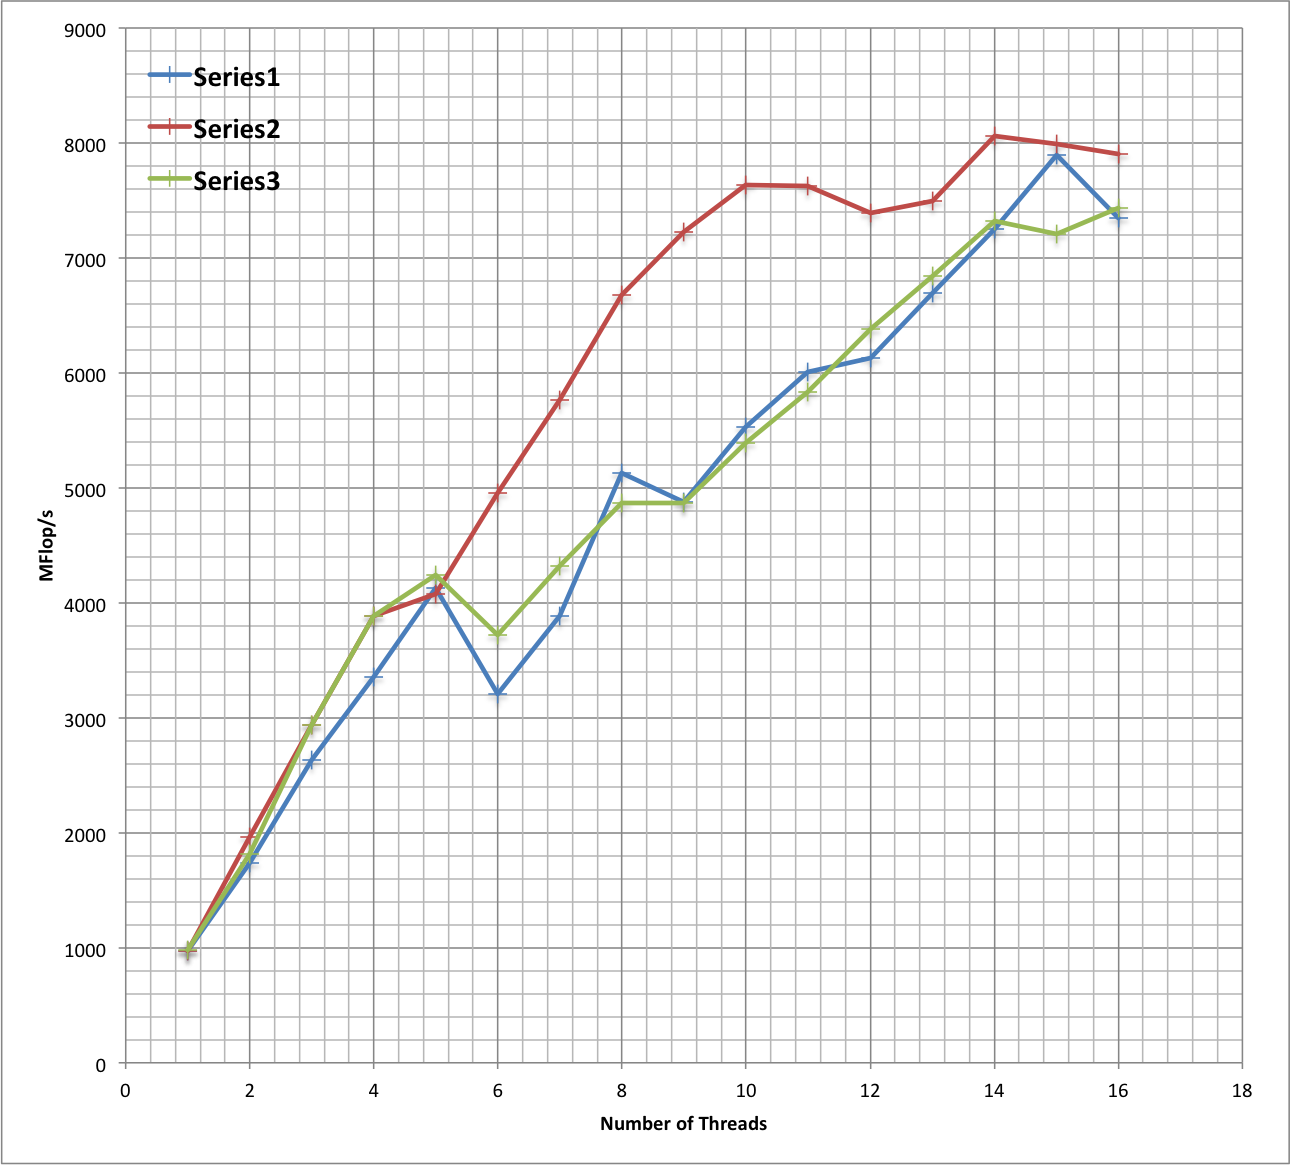
\includegraphics[width=0.8\textwidth]{mat_mul_scale.png}
\caption{series 1: omp for; series 2: omp task; series 3: pThreads}
\label{fig:awesome_image}
\end{figure}

\subsection{Peak Performance}
I changed the for loop ordering for all matrix multiply implementation to make the process a little faster. So, the scalar baseline was $970MFlop/s$ and the best parallel performance was $8060MFlop/s$ with 14 threads using the OpenMP task implementation. Hence, the speed-up was $8.3$ time faster than the baseline. 

\noindent No, we are not achieving linear speed-up. The speed-up is about $0.86$ performance improvement per thread for the first ten threads. For the runs of 1 thread through 10 threads the performance increases linearly. However, it is not an ideal linear scaling as the speed-up is less then 1 performance improvement per thread. And also the performance starts flattening out by running the program on 11 through 16 threads.

\noindent The OpenMP Task implementation is the one that performs the best because it deals better with load balancing, namely faster threads do not remain idle while waiting for slower threads to complete execution. 


\subsection{Measuring up peak performance}
The peak performance achieved by our algorithm is $8.06$ GigaFlops/s, which is about $9.5$ slower than the peak performance of one hive machine. This is because our algorithm only exploits multiple threads of execution, but does not exploit memory optimisations and SSE intrinsics. I would do some loop unrolling, reorder the loops so that I can load some values out of the inner loop and save them on some register, and use SSE intrinsics to do multiple instructions at the same time.


\subsection{Preference}
I like OpenMP better because it is much more productive that pThreads. Id est development is faster because a lot is done for you already, and there is less risk to shoot yourself in the foot compared to pThreads. However, sometimes I prefer to have more control on how my threads are being utilised and for that I would use pThreads.

\subsection{How does OpenMp work}
OpenMP is a high level abstraction that uses pThreads under the hood. When the -fopenmp flag is activated the compiler transforms the source code into multithreaded code (like in the example below), and follows roughly the following steps:
\begin{enumerate}
\item Reads and parses OpenMP directives, and checks for correctness
\item Translates SECTIONs to DO/FOR statements
\item Makes implicit barriers explicit
\item Implements some optimisations like merging adjacent parallel regions
\item Implements variable data attributes, sets up storage and range for initialisation
\end{enumerate}
\begin{lstlisting}[label=some-code,caption=Original Code]
#pragma omp for
for( i = 0; i < n; i++ ) 
{ �}
\end{lstlisting}

\begin{lstlisting}[label=some-code,caption=Transformation]
tid = ompc_get_thread_num();
ompc_static_init (tid, lower,upper, 
incr,.); 
for( i = lower;i < upper;i += incr ) 
{ � }
// Implicit BARRIER
ompc_barrier();
\end{lstlisting}

\pagebreak

\section{Two-Dimensional Convolution}

\subsection{Scaling Plots}

\begin{figure}[h]
\centering
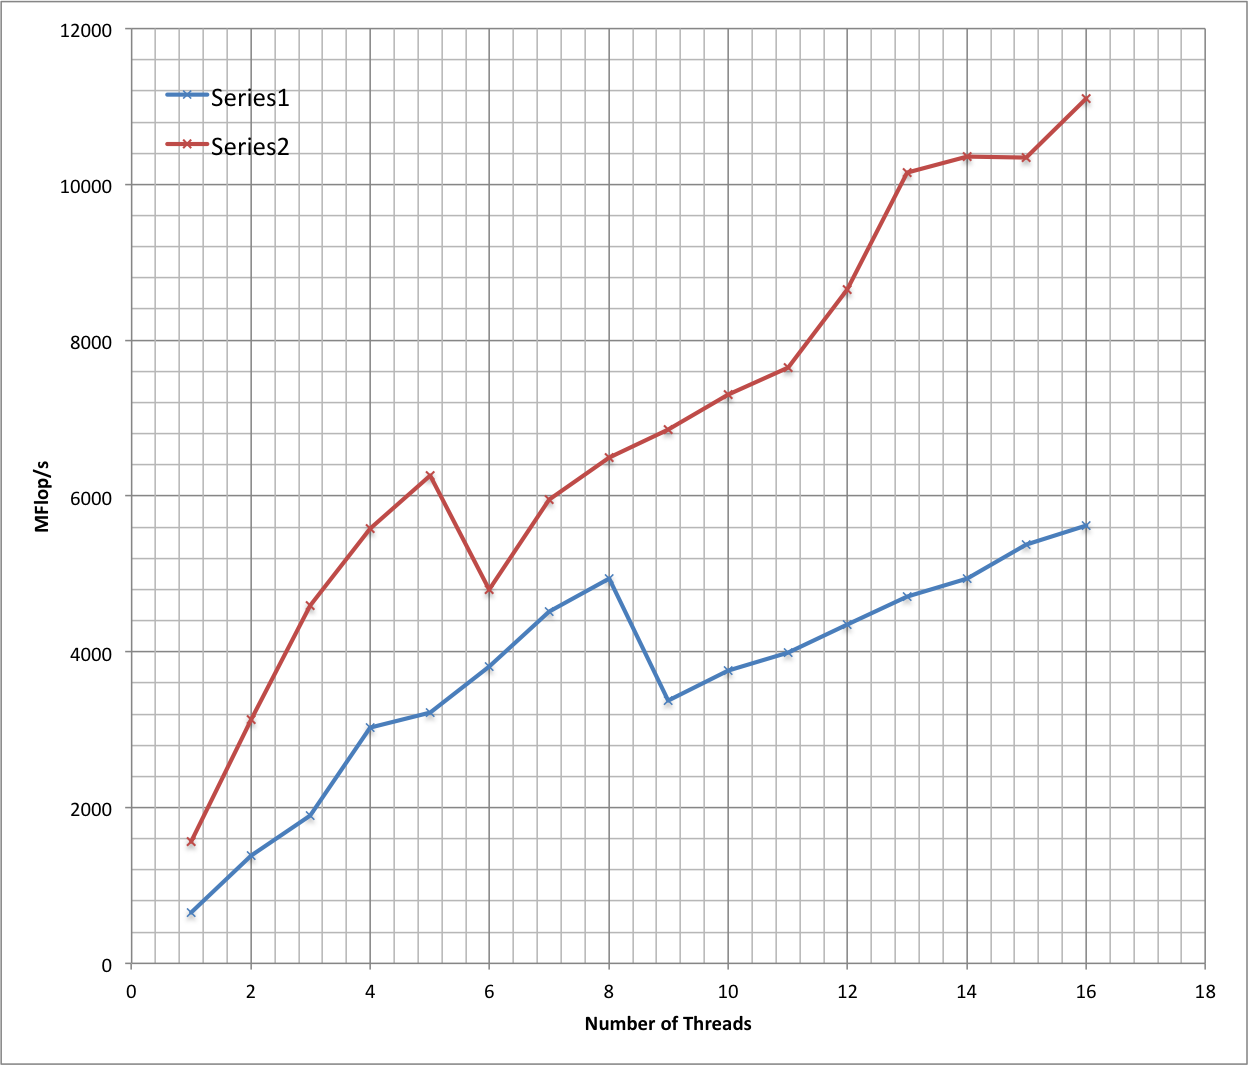
\includegraphics[width=0.8\textwidth]{conv2d_scale.png}
\caption{series 1: -n1; series 2: -n10}
\label{fig:awesome_image}
\end{figure}


\subsection{Comments On Scaling Performances}
The code scales better with maximum radius 10. This could be due to the fact that we exploit more spatial locality in the radius loops. We could improve performance by coin multiple operations with SSE intrinsics. For example when the blur radius is even.
\subsection{Time spent on assignment}
About 4 hours...





%\begin{lstlisting}[label=some-code,caption=Random Permutation with 1 cycle]

%\end{lstlisting}


%\begin{figure}[h]
%\centering
%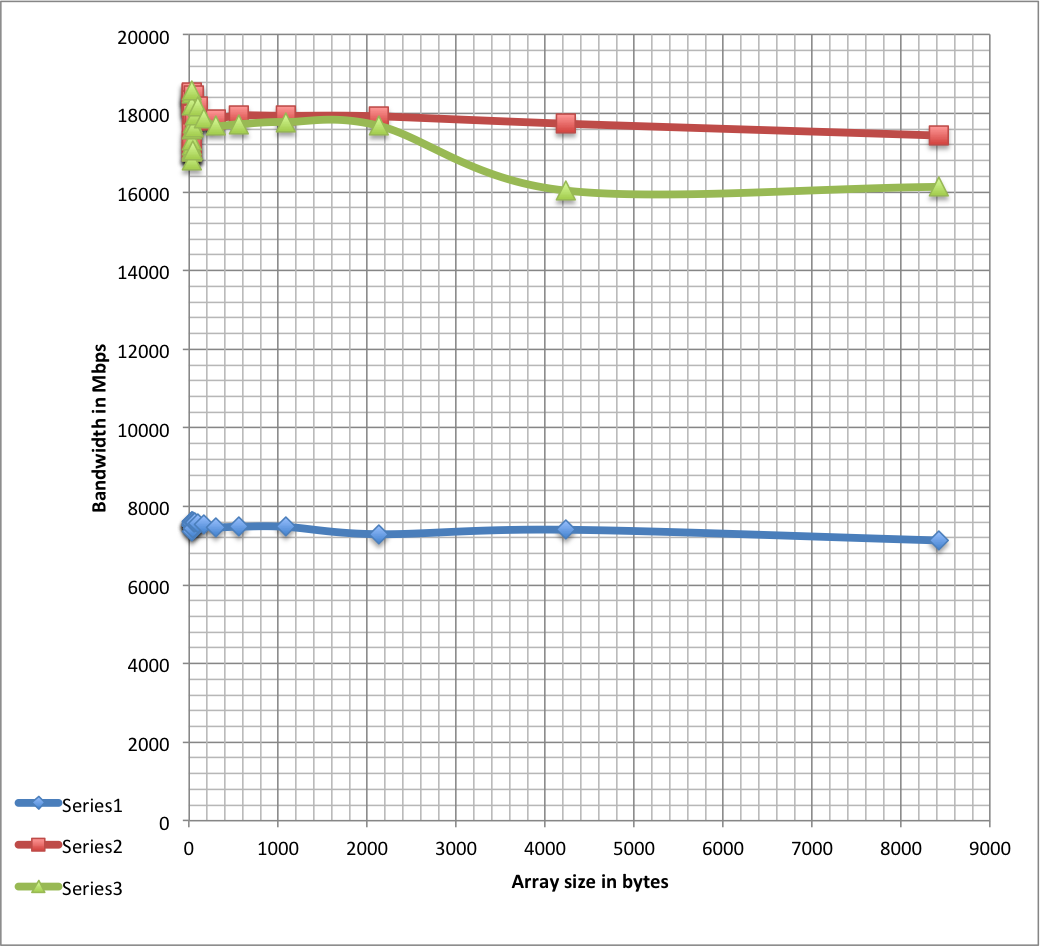
\includegraphics[width=0.8\textwidth]{graph_mem.png}
%\caption{series 1: inefficient routine; series 2: simd\_memcpy; series 3: simd\_memcpy\_cache}
%\label{fig:awesome_image}
%\end{figure}



\end{document}








% \begin{lstlisting}[label=some-code,caption=Some Code]
% public void here() {
% goes().the().code()
% }
% \end{lstlisting}








